%% -----------------Fracture toughness (CAU Kiel)
\subsection{Fracture Toughness of the Opalinus Claystone}
\label{sec:Fracture_Toughness_Exp}
\Authors{Amir Shoarian Sattari (CAU)}
%\todo{Please insert authors}

In linear elastic fracture mechanics, a materials resistance to fracture propagation is known as fracture toughness. The unit of the fracture toughness is $Pa.\sqrt m$ and the fracture toughness is measured under coupled or individual three different fracture modes I, II and III. In a three-point bending test, the flexural strength ($\sigma_{flex}$), flexural Young's modulus ($E_{flex}$) and flexural strain ($\epsilon_{flex}$) parameters are measured. The fracture toughness test using the three-point bending test provides the Mode I fracture toughness ($K_{Ic}$) of the material (Fig.  \ref{fig:Amir_Fracture_Toughness_Theory}).
\index{fracture toughness}
\index{three-point bending test}

\begin{figure}[!ht]
\centering
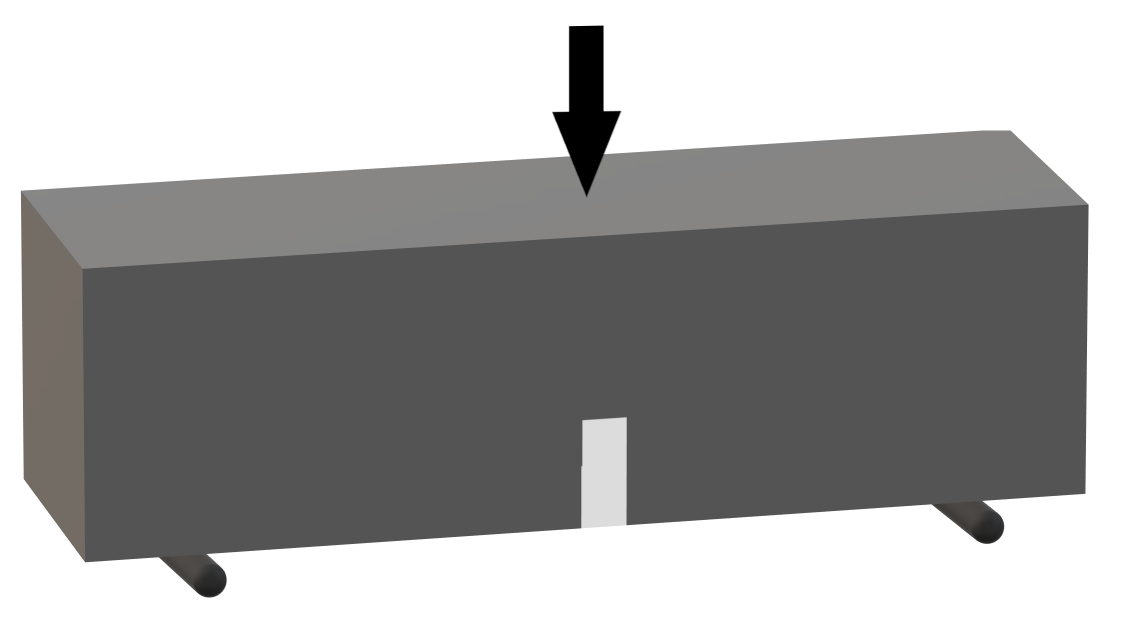
\includegraphics[width=6cm,height=3cm]{figures/Amir_Fracture_Toughness_Theory.png}
\caption{The fracture toughness assessment using three-point bending test}
\label{fig:Amir_Fracture_Toughness_Theory}
\end{figure} 

The stress intensity factor ($K_I$) on the crack tip of predefined notch is obtained with equation (\ref{eq:Fracture_Toughness}) \cite{Bower2009},

\begin{multline}
\label{eq:Fracture_Toughness}
K_I=
\frac{4f_{flex}}{B_{flex}}
\sqrt{\frac{\pi}{W_{flex}}}
\left(1.6
\left(\frac{a_{flex}}{W_{flex}}\right)^\frac{1}{2}
-
2.6\left(\frac{a_{flex}}{W_{flex}}\right)^\frac{3}{2} 
\right.
\\ 
\left.
+12.3\left(\frac{a_{flex}}{W_{flex}}\right)^\frac{5}{2} -21.2\left(\frac{a_{flex}}{W_{flex}}\right)^\frac{7}{2}
+21.8\left(\frac{a_{flex}}{W_{flex}}\right)^\frac{9}{2}
\right)
\end{multline}

where, $f_{flex}$ is the flexural load, $a_{flex}$ is the length of the pre-defined notch, $B_{flex}$ and $W_{flex}$ are the thickness and height of the sample under the flexural test, respectively. During the test procedure, the load and crack mouth opening displacement (CMOD) values are measured and plotted. At the load in which the crack starts to propagate into the medium the fracture toughness $K_{Ic}$ is calculated. In order to perform the fracture toughness test, a loading cell with three rolling supports is required (Fig. \ref{fig:Amir_Fracture_Toughness_Setup_a}). However, the in-situ condition can only be reached when a material is under controlled temperature and humidity conditions. Therefore, a climate chamber in a laboratory of CAU Kiel has been utilized to reach the desired temperature and humidity (Fig. \ref{fig:Amir_Fracture_Toughness_Setup_b}). The temperature can be controlled between 20 to 80 $^{\circ}C$ and relative humidity varies from 0 up to 100. 
\index{crack mouth opening displacement (CMOD)}

\begin{figure}[!ht]
\centering
\begin{subfigure}[c]{0.6\textwidth}
\centering
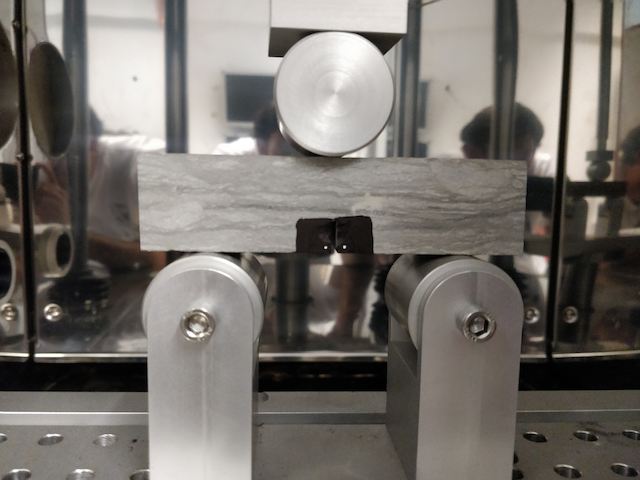
\includegraphics[width=6cm,height=5cm]{figures/Amir_Fracture_Toughness_Setup_a.png}
\subcaption{}
\label{fig:Amir_Fracture_Toughness_Setup_a}
\end{subfigure}
\begin{subfigure}[c]{0.38\textwidth}
\centering
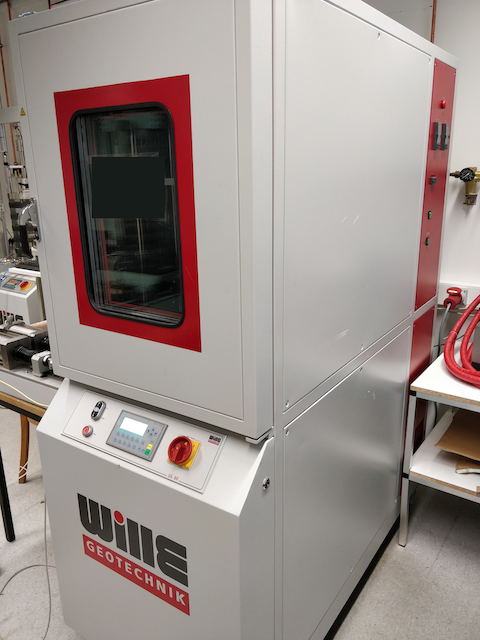
\includegraphics[width=4cm,height=5cm]{figures/Amir_Fracture_Toughness_Setup_b.png}
\subcaption{}
\label{fig:Amir_Fracture_Toughness_Setup_b}
\end{subfigure}
\caption{The required equipment for performing the three-point bending test (a) the loading cell and supports, (b) the climate chamber for controlling temperature and humidity}
\end{figure}

The claystone samples are prepared with the dimension of 140x30x30 $(mm)$ and the notch dimension of 2x10x30 $(mm)$v $(LxWxB)$  (Fig.\ref{fig:Amir_Fracture_Toughness_Sample}). The span length ($S_{flex}$) is 120 $mm$, which is 4 times the size of its width and thickness. The embedded layering is perpendicular to the loading direction. The image processing technique is used to track the reference points, which are predefined prior to the test procedure (Fig. \ref{fig:Amir_Fracture_Toughness_Image_a}). The distance between the points is measured using the optical microscopic image and is considered as an initial reading value (Fig. \ref{fig:Amir_Fracture_Toughness_Image_b}). The method is able to detect the minimum displacement of 2 micrometers, which is possible by taking 4k video with 30fps. The load vs. CMOD response of the Opalinus claystone as well as the numerical simulation outcomes are given in \ref{sec:mex01}. The effects of anisotropy and embedded layering orientation of Opalinus claystones on fracture toughness values are not fully studied. 

\begin{figure}[!ht]
\centering
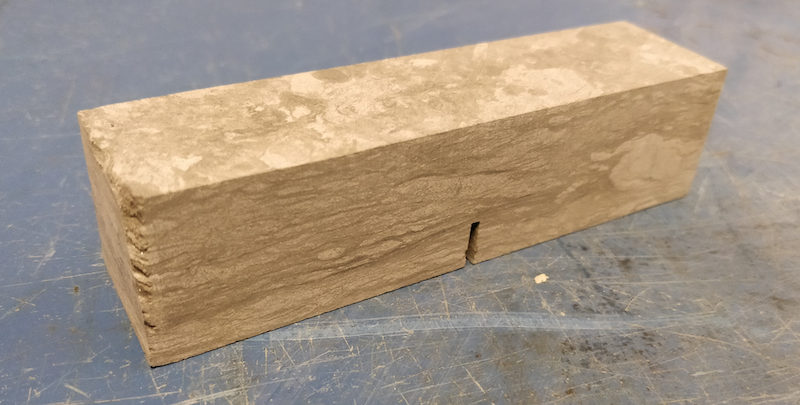
\includegraphics[width=8cm,height=4cm]{figures/Amir_Fracture_Toughness_Sample.png}
\caption{The prepared Opalinus claystone sample with the dimension of 140x30x30 $mm$}
\label{fig:Amir_Fracture_Toughness_Sample}
\end{figure} 

\begin{figure}[!ht]
\centering
\begin{subfigure}[c]{0.48\textwidth}
\centering
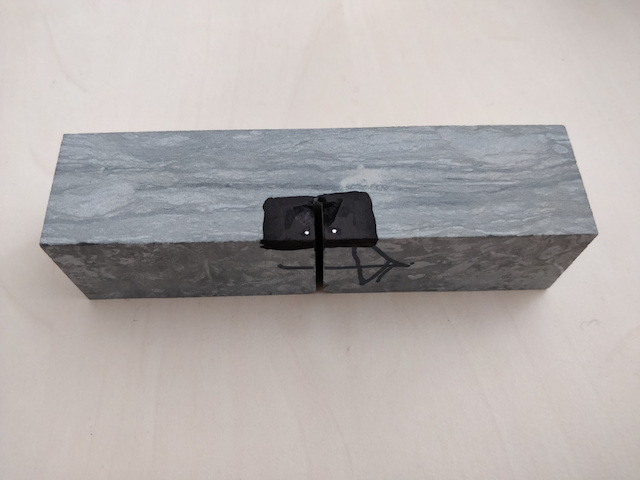
\includegraphics[width=6cm,height=5cm]{figures/Amir_Fracture_Toughness_Image_a.png}
\subcaption{}
\label{fig:Amir_Fracture_Toughness_Image_a}
\end{subfigure}
\hfill
\begin{subfigure}[c]{0.48\textwidth}
\centering
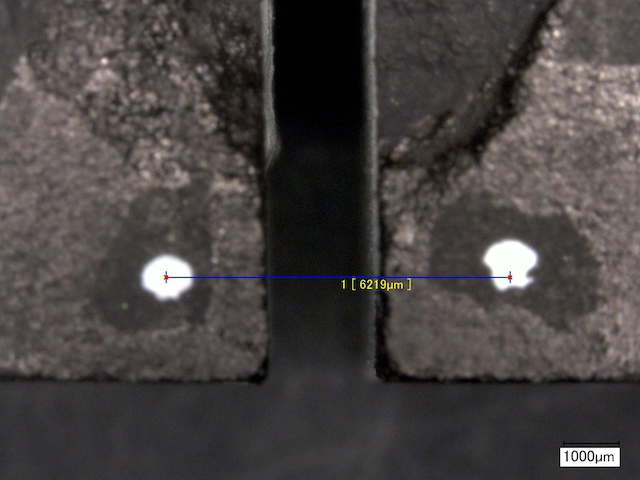
\includegraphics[width=6cm,height=5cm]{figures/Amir_Fracture_Toughness_Image_b.png}
\subcaption{}
\label{fig:Amir_Fracture_Toughness_Image_b}
\end{subfigure}
\caption{The application of image processing technique (a) the predefined reference points for measuring the CMOD, (b) the measured rough distance using optical microscope}
\end{figure}